\documentclass[a4paper,12pt,liststotoc,DIV12]{scrartcl}
%\usepackage{geometry}
%\usepackage{ngerman}
\usepackage{longtable}
\usepackage[T1]{fontenc}
\usepackage{ae}
\usepackage[utf8]{inputenc}
\usepackage{fancyhdr}
\usepackage{fancyvrb}
\usepackage{graphicx}
\usepackage{xspace}
\usepackage[cmyk]{xcolor}
\usepackage{amsmath}
\usepackage{url}
\usepackage[
  %plainpages=false,
  %pdfpagelabels,
  %colorlinks=true,
  pdfborder={0 0 0},
  %urlcolor=blue,
  %linkcolor=blue,
  bookmarksopen=true,
  %pdfstartpage=3,
  unicode,
]{hyperref}
\hypersetup{
  pdftitle={OST-WeST - Design},
  pdfsubject={OST-WeST - Design},
  pdfauthor={Stefan Franke, Robert Hanussek, Benjamin Keil, Steffen Kieß, Johannes Langauf, Christoph Marian Müller, Igor Podolskiy, Tilmann Scheller, Michael Starzmann, Markus Wittlinger},
  pdfkeywords={OST-WeST, Design},
}
% hypcap is needed for correct links to figures, see specification Bug 2
\usepackage[all]{hypcap}
\usepackage{svnkw}
\usepackage[USenglish]{isodate}
\usepackage{titlesec}
% provides \ul,  allows line breaking for underlined text (static methods...)
\usepackage{soul}
\makeatletter

% some TeX voodoo to extract the date from SVN ID
% which can be processed by isodate 
\def\svn@dateonly#1 #2Z{#1}
\def\svndateonly#1{%
\ifx#1\empty1970-01-01\else
\expandafter\svn@dateonly#1\fi}

% Two-level figure & table numbering
\@addtoreset{table}{section}
\@addtoreset{figure}{section}
\renewcommand{\thefigure}{\thesection.\arabic{figure}}
\renewcommand{\thetable}{\thesection.\arabic{table}}
\makeatother

% custom font sizes for headings, non run-in titles for [sub]paragraphs
\titleformat{\section}{\bfseries\fontsize{24}{30}\selectfont\sffamily}{\thesection}{1em}{}
\titleformat{\subsection}{\bfseries\fontsize{18}{24}\selectfont\sffamily}{\thesubsection}{1em}{}
\titleformat{\subsubsection}{\bfseries\fontsize{16}{22}\selectfont\sffamily}{\thesubsubsection}{1em}{}
\titleformat{\paragraph}{\bfseries\fontsize{14}{20}\selectfont\sffamily}{\theparagraph}{1em}{}
\titleformat{\subparagraph}{\bfseries\normalsize\sffamily}{\thesubparagraph}{1em}{}
\titlespacing{\paragraph}{0pt}{\parskip}{-0.5\parskip}{}
\titlespacing{\subparagraph}{0pt}{\parskip}{-0.5\parskip}{}

\svnid{$Id$}

\parindent0mm
\parskip2mm
%\geometry{textwidth=160mm, textheight=230mm, inner=30mm}

\xdefinecolor{TodoColor}{rgb}{1.0, 0.0, 0.0}

% depth of the headlines that are numbered
\setcounter{secnumdepth}{5}
\setcounter{tocdepth}{5}

\newcommand{\OSTWeST}{\textit{OSTWeST}\xspace}
\newcommand{\gbt}{\textit{CodeCover}\xspace}
\newcommand{\eclui}{\textsf}
\newcommand{\code}{\texttt}
\newcommand{\todo}[1]{\bgroup\color{TodoColor}\textsc{\textbf{TODO:} #1}\egroup}
\newcommand{\BIG}{\fontsize{48}{48}\selectfont}
\newcommand{\linkwithfootnote}[2]{\href{#1}{#2}\footnote{\url{#1}}}
\newcommand{\email}[1]{\href{mailto:#1}{#1}}

\xdefinecolor{ClassColor}         {rgb}{0.0, 1.0, 0.0}
\xdefinecolor{ClassAbstractColor} {rgb}{0.0, 1.0, 0.0}
\xdefinecolor{ObjectColor}        {rgb}{0.31, 0.58, 0.84}
\xdefinecolor{InterfaceColor}     {rgb}{1.0, 0.0, 1.0} % that's magenta NOT pink, OK? ;-)
\xdefinecolor{ImplementerColor}   {rgb}{0.4, 0.2, 0.6}
\xdefinecolor{FieldColor}         {rgb}{0.9, 0.5, 0.0}

\newcommand{\pkg}[1]{\url{#1}}
\newcommand{\cls}[1]{\texorpdfstring{{\color{ClassColor}\url{#1}}}{#1}}
\newcommand{\clsab}[1]{\texorpdfstring{{\color{ClassAbstractColor}\textit{\url{#1}}}}{#1}}
\newcommand{\obj}[1]{\texorpdfstring{{\color{ObjectColor}\url{#1}}}{#1}}
\newcommand{\itf}[1]{\texorpdfstring{{\color{InterfaceColor}\url{#1}}}{#1}}
\newcommand{\imp}[1]{\texorpdfstring{{\color{ImplementerColor}\url{#1}}}{#1}}
\newcommand{\mtd}[1]{\url{#1}}
\newcommand{\mtdst}[1]{\texorpdfstring{\url{#1}}{#1}}
\newcommand{\mtdab}[1]{\texorpdfstring{\textit{\url{{#1}}}}{#1}}
\newcommand{\fld}[1]{{\color{FieldColor}\url{#1}}}
\newcommand{\namespace}[1]{\begin{description}\item[Namespace:]#1\end{description}}
\newcommand{\rootpkg}{org.codecover}

\newcommand{\codepageflag}{iscodecontainer}

% needed for the Function Point tables
\newcommand{\x}{\textbullet}

% needed for the ConditionCoverageApproach2
\xdefinecolor{UnInstrumentedColor}{rgb}{0.9, 0.2, 0.0}
\xdefinecolor{DepthA}{rgb}{0.9, 0.0, 0.0}
\xdefinecolor{DepthB}{rgb}{0.0, 0.0, 0.9}
\xdefinecolor{DepthC}{rgb}{0.0, 0.3, 0.6}
\xdefinecolor{DepthD}{rgb}{0.0, 0.6, 0.3}
\xdefinecolor{DepthE}{rgb}{0.0, 0.9, 0.0}

\newcommand{\uic}[1]{\textcolor{UnInstrumentedColor}{#1}\xspace}
\newcommand{\depAo}{\textcolor{DepthA}{(}}
\newcommand{\depAc}{\textcolor{DepthA}{)}}
\newcommand{\depBo}{\textcolor{DepthB}{(}}
\newcommand{\depBc}{\textcolor{DepthB}{)}}
\newcommand{\depCo}{\textcolor{DepthC}{(}}
\newcommand{\depCc}{\textcolor{DepthC}{)}}
\newcommand{\depDo}{\textcolor{DepthD}{(}}
\newcommand{\depDc}{\textcolor{DepthD}{)}}
\newcommand{\depEo}{\textcolor{DepthE}{(}}
\newcommand{\depEc}{\textcolor{DepthE}{)}}

%\includeonly{Introduction}
%\includeonly{UserInterface}
%\includeonly{FunctionalRequirements}
%\includeonly{NonFunctionalRequirements}
%\includeonly{Conclusion}
%\includeonly{ConditionalCoverageProof}
%\includeonly{CoverageLogFileSpecification}
\begin{document}

% --- title page --- %
\pagestyle{empty}
\begin{titlepage}
 \vspace*{38mm}
 \begin{center}
 \fontsize{24}{24}\selectfont
 Design\\
 \vspace*{12mm}
 \fontsize{48}{48}\selectfont
 
 % gross hack to generate the a big fancy gbt-squared appearance
 \textit{CodeCover}
 %
 \\
 \fontfamily{\familydefault}\fontsize{32}{38}\selectfont
 Glass Box Testing Tool\\
 \vspace*{12mm}
 \fontsize{16}{20}\selectfont
 Student Project A ``OST-WeST''\\
 University of Stuttgart

 \vspace{2cm}
 {\small 
   Version: 1.2 \\
   {Last changed on \printdate{\svndateonly{\svndate}} (SVN Revision \svnrev)}}
   \end{center}
   \vspace{3cm}
   \hspace{40mm}
   \normalsize
\end{titlepage}

% --- Header and version history --- %

\cleardoublepage
\fancyhf{}
\fancyhead[RE,LO]{\textit{\gbt - Design}}
\fancyhead[RO,LE]{\thepage}
\pagestyle{fancyplain}

% --- Table of contents --- %

\parskip1mm
\tableofcontents
\parskip2mm

\pagestyle{fancyplain}
\renewcommand{\baselinestretch}{1.25}\normalsize
\svnid{$Id$}
\section{Introduction} \label{Introduction}

\subsection{Project overview} \label{in:Overview}
\gbt stands for \textbf{g}lass \textbf{b}ox \textbf{t}esting \textbf{t}ool. It measures the \gl[code coverage]{code coverage} of a running program and will be as independent as possible of the programming language of the covered program.
\par
Characteristics of \gbt:
\begin{itemize}
  \item \gbt runs at least on Linux and Windows,
  \item \gbt can measure code coverage for programs written in Java and COBOL.
  \item \gbt is extensible to measure code coverage for further programming languages as well.
  \item \gbt measures multiple code coverage criteria and is extensible to further ones.
  \item \gbt provides functionality to create reports of the measured code coverage in \gl[HTML]{HTML}-files.
  \item \gbt is an Eclipse\linkwithfootnote{http://www.eclipse.org/}{} plug-in with a graphical user interface, but also provides a command line interface for use without Eclipse.
\end{itemize}
\par
To understand the functional requirements specified in this document, a visual overview of the work flow is shown in figure~\ref{in_fg:Workflow of the software}.
\begin{figure}[hbtp]
 \centering
 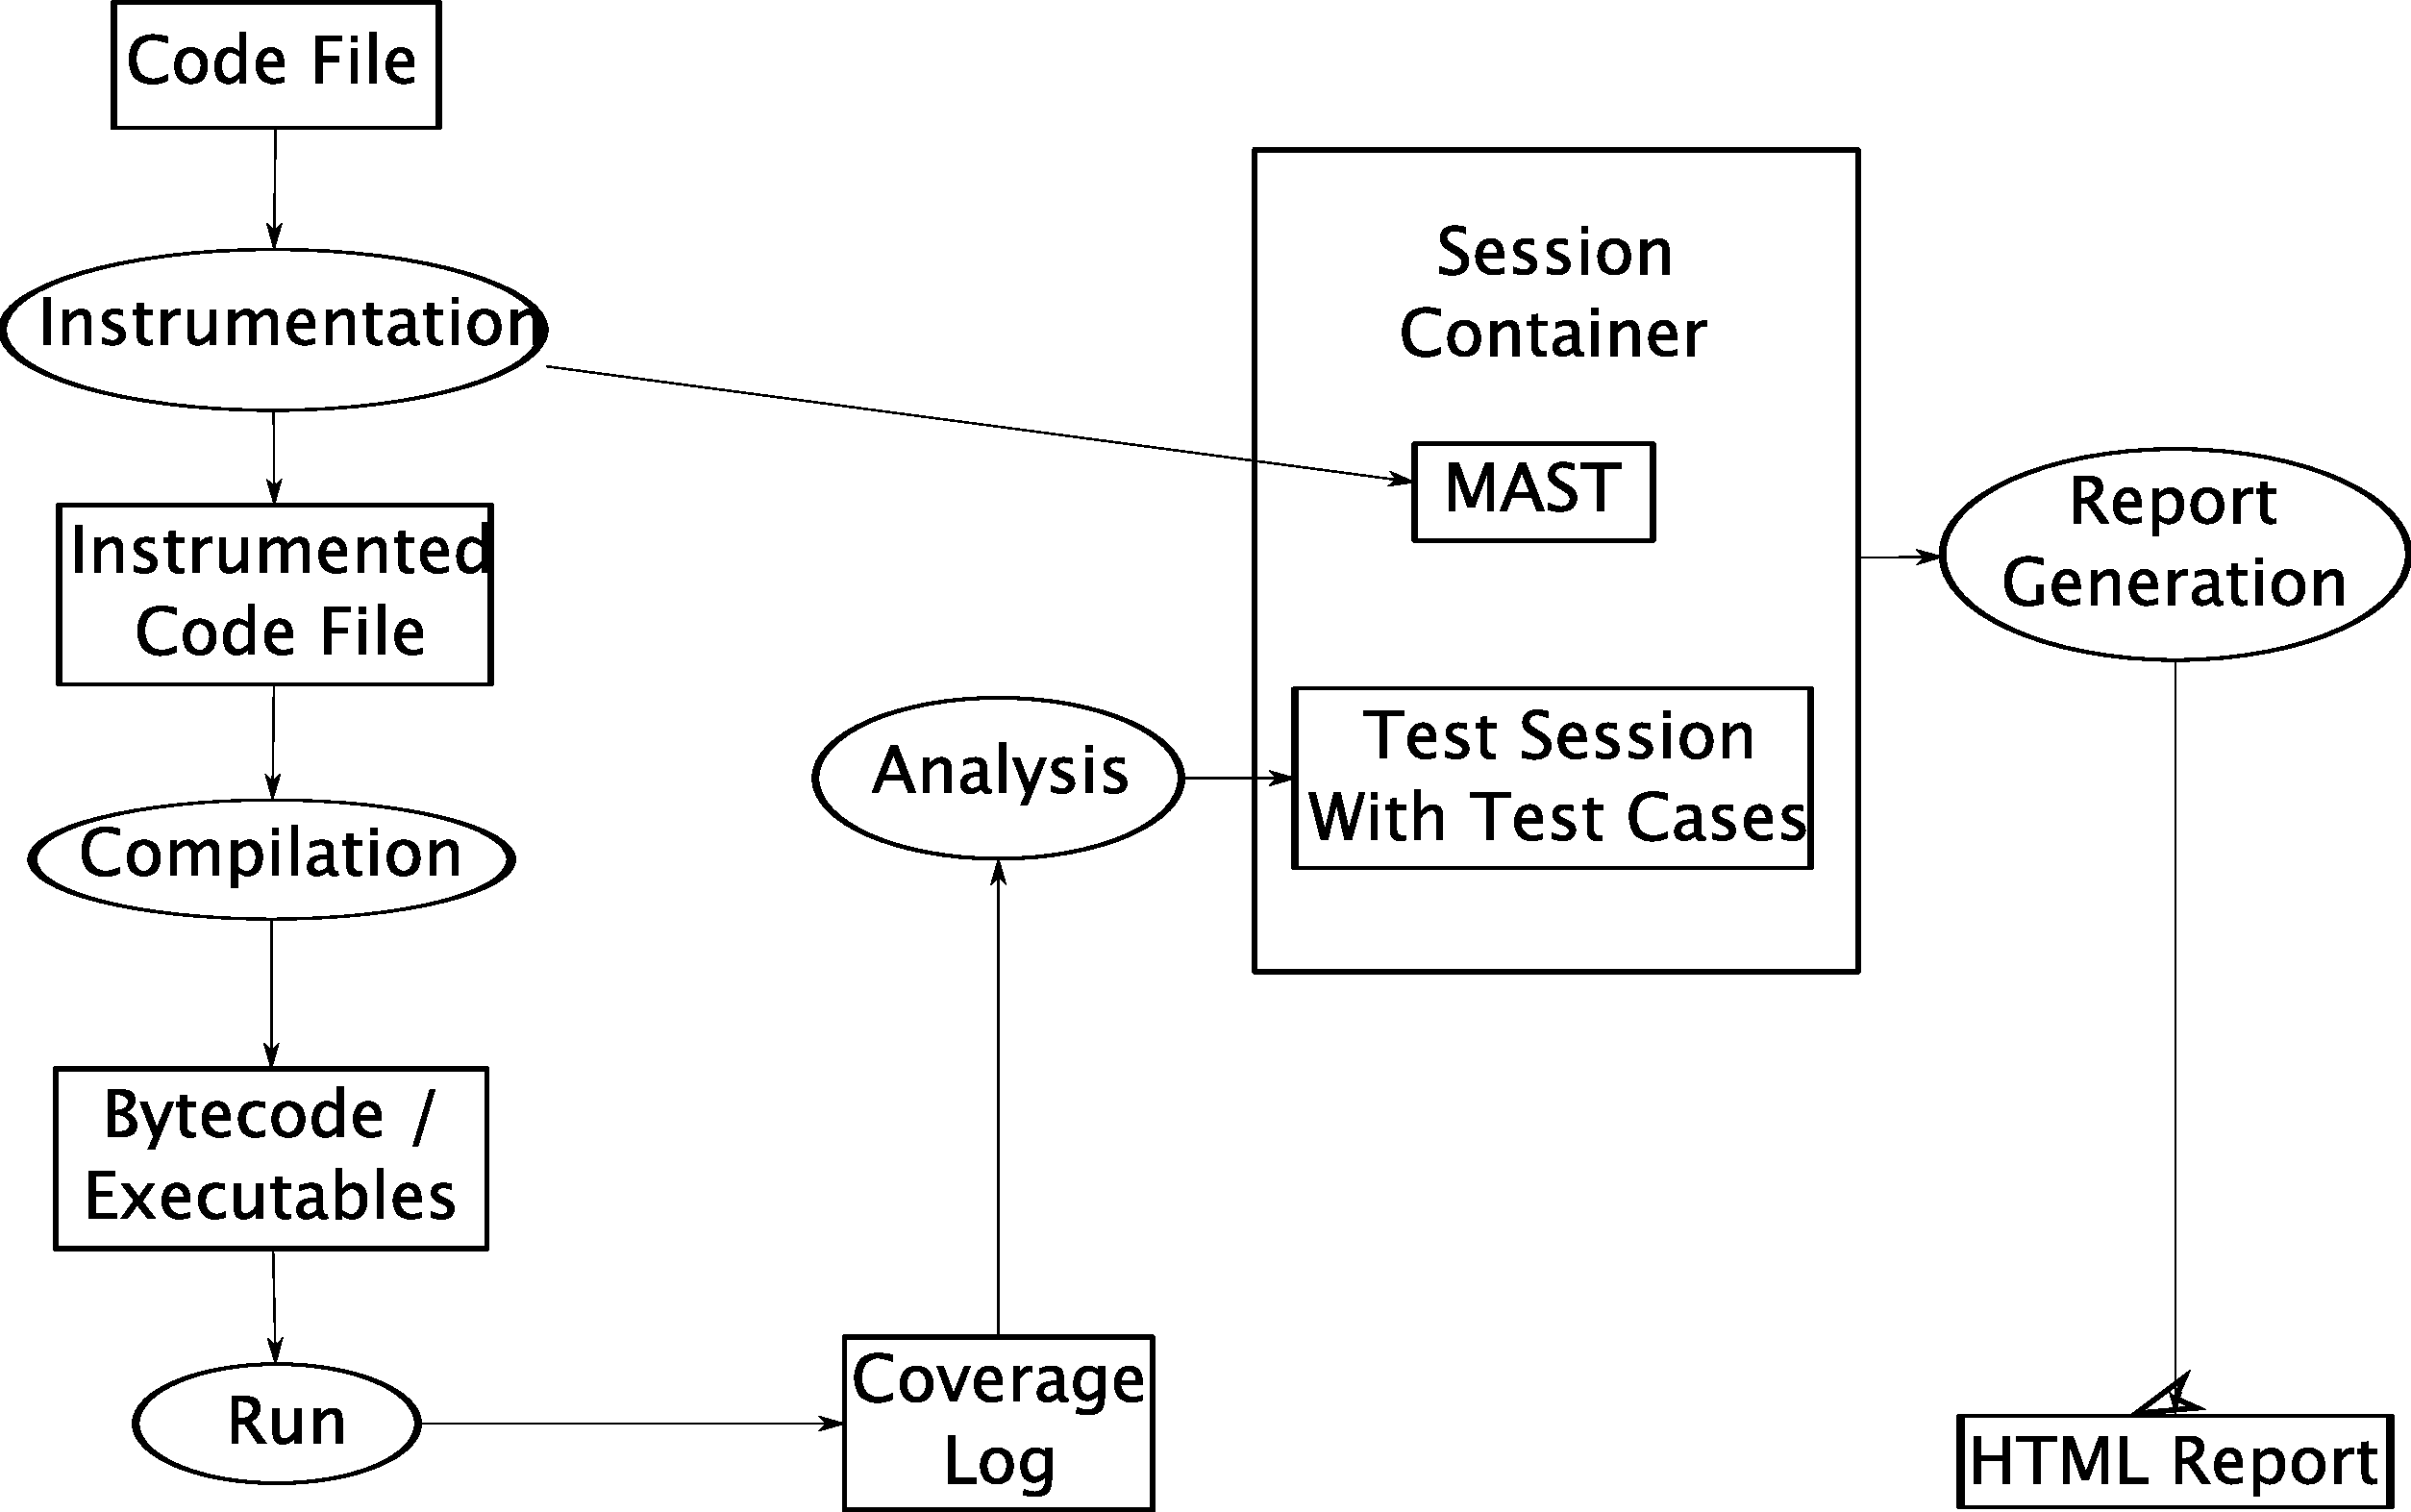
\includegraphics[width=0.7\textwidth]{images/Workflow/Workflow}
 \caption{Work flow of the software}
 \label{in_fg:Workflow of the software}
\end{figure}
\par
Several steps and intermediate results exist for the whole of the coverage measurement process. The ellipses stand for processing, the rectangles stand for intermediate results or final results.
\par
The process starts with the \gl[instrumentation]{instrumentation} of \gl[code file]{code files}. A \gl{MAST} is produced in addition to the instrumented code files. The \gl{MAST} is stored with the \gl[code file]{code files} in a \gl{session container}. After the compilation and execution of all the instrumented code files of the \gl[SUT]{SUT}, a \gl[coverage log]{coverage log} with the raw coverage results is produced.
\par
During the analysis phase, the coverage log is processed to obtain a \gl[test session]{test session} with \gl[test case]{test cases}. They contain all the processed coverage results. These information are added to the \gl{session container}.
\par
Using the information of the \gl{MAST} and the \gl[test session]{test sessions}, \gbt can generate a \gl[HTML]{HTML} report.

\subsection{About this document} \label{in:AboutThisDocument}
This document specifies all requirements the software has to fulfill and all interfaces to users or other programs. The design of the software will be written based upon this document. This document is the common ground between the customer and the \gl[developer]{developers}. Therefore, it's important that both, customers and developers, pay attention to the quality of this document and keep it current.

\subsection{Addressed audience} \label{in:Addressed audience}
This document is addressed to
\begin{itemize}
  \item the customer who ordered the software
  \item the project manager controlling the work
  \item the designers writing the software design
  \item the quality assurance division creating \gl[test case]{test cases} for the software
  \item the developers implementing the design
  \item future developers maintaining and extending the software
  \item interested users of the software
  \item students of upcoming student projects
\end{itemize}

\subsection{Conventions for this document} \label{in:Conventions for this document}
A glossary is shipped together with this \gl[specification]{specification}. It contains basic definitions and allows clear statements in this document because it prevents ambiguity. Therefore words mentioned in the glossary are used often and are not explicitly defined in this specification but in the glossary.
\par
The term ``software'' is used for \gbt. Code examples and file names are written in the \code{typewriter style}. Labels and names of graphical user interface components are written in \eclui{small caps}. If necessary, examples are used and placeholders are enclosed by percentage signs: \%placeholder\%. Furthermore, glossary entries are marked with the symbol $\nearrow$, but only at the first occurrence in a section.

\subsection{Authors}
In the following table the contact persons per section are named.
{\small
\begin{longtable}{|p{35mm}|p{35mm}|l|} \hline
   {\normalsize \textbf{Section}} &
   {\normalsize \textbf{Author}} &
   {\normalsize \textbf{E-mail}} \\\hline \hline \endhead
   Introduction & Michael Starzmann & starzmml@studi.informatik.uni-stuttgart.de \\\hline
   Functional requirements (\ref{fr:Test sessions and test cases} -- \ref{fr:Configuration}) & Christoph Müller & muellecr@studi.informatik.uni-stuttgart.de \\\hline
   Functional requirements (\ref{fr:Report} -- \ref{fr:Language support}) & Michael Starzmann & starzmml@studi.informatik.uni-stuttgart.de \\\hline
   Graphical user interface & Stefan Franke & frankesn@studi.informatik.uni-stuttgart.de \\\hline
   Non-functional requirements & Johannes Langauf & langaujs@studi.informatik.uni-stuttgart.de \\\hline
\end{longtable}
}
%%% Local Variables: 
%%% mode: latex
%%% TeX-master: "Specification.ltx"
%%% End: 

\svnid{$Id$}
\section{UML-Model}
\linkwithfootnote{http://bouml.free.fr}{BOUML 2.21.5} was used to create the UML-Model. The BOUML files can be found in the subversion repository under \code{/svn/trunk/design/design/}. To avoid inconsistencies between this document and the model detailed in BOUML, no diagrams are included here, but all exist within the model. 
\section{Code examples}
Examples for instrumented Java- and COBOL-Code can be found in the subversion repository under \code{/svn/trunk/misc/instrumentation/code\_examples/}. The content of these files is not included here, because code examples are cumbersome and better readable in a normal text editor or IDE.
\section{Structural makeup of XML-Files}
\begin{verbatim}
<HierarchyLevel>
	<HierarchyLevelType englishName="" internalName=""/>
	<LocationList>
		<Location startOffset="" endOffset="">
			<SourceFile fileName="" content=""/>
		</Location>
	</LocationList>
	<StatementSequence>
		<BasicStatement>
			<CoverableItem id=""/>
			<RootTerm>
				<MapEntry>
					<BooleanAssignment>
						<BooleanResult value=""/>
						<BooleanResult value=""/>							<BooleanResult value=""/>
					</BooleanAssignment>
					<CoverableItem id=""/>
				</MapEntry>
				<BooleanTerm type="">
					<BooleanTerm type="">
					<BooleanOperator arity="" name=""/>
						<MapEntry>
							<BooleanAssignment>
								<BooleanResult value=""/>
								<BooleanResult value=""/>								<BooleanResult value=""/>
							</BooleanAssignment>
							<Boolean value="">
						</MapEntry>
					</BooleanTerm>
				</BooleanTerm>
			</RootTerm>
		</BasicStatement>
		<LoopingStatement optionalBodyExecution="" neverExecutedItemId="" onceExecutedItemId="" multipleExecutedItemId="">
			<LocationList>
				<Location startOffset="" endOffset="">
					<SourceFile fileName="" content=""/>
				</Location>
			</LocationList>
			<CoverableItem id=""/>
			<RootTerm/>
			<StatementSequence/>
		</LoopingStatement>
		<ConditionalStatement>
			<LocationList>
				<Location startOffset="" endOffset=""/>
					<SourceFile fileName="" content=""/>
				</Location>
			</LocationList>
			<Branch implicit="">
				<Location startOffset="" endOffset="">
					<SourceFile fileName="" content=""/>
				</Location>
				<CoverableItem id=""/>
			</Branch>
			<RootTerm/>
			<StatementSequence/>
		</ConditionalStatement>
	</StatementSequence>
	<HierarchyLevel/>
</HierarchyLevel>
				
\end{verbatim}


% --- List of figures --- %

\newpage
% \phantomsection is needed for correct PDF link to the LOF
% (see specification Bug 2)
\phantomsection
\listoffigures
%\addcontentsline{toc}{section}{List of figures}

\begin{appendix}
\documentclass[a4paper,12pt,DIV12]{scrartcl}
\usepackage{longtable}
\usepackage[T1]{fontenc}
\usepackage{ae}
\usepackage[utf8]{inputenc}
\usepackage{fancyhdr}
\usepackage{fancyvrb}
\usepackage{xspace}
\usepackage[cmyk]{xcolor}
\usepackage{amsmath}
\usepackage[
  pdfborder={0 0 0},
  pdftitle={OST-WeST - Formal Proof Of Conditional Coverage Instrumentation},
  pdfsubject={OST-WeST - Formal Proof Of Conditional Coverage Instrumentation},
  pdfauthor={Christoph Marian Müller},
  pdfkeywords={OST-WeST, Formal Proof Of Conditional Coverage Instrumentation},
  bookmarksopen=true,
]{hyperref}
\usepackage{svnkw}
\usepackage[USenglish]{isodate}
\usepackage{titlesec}

\parindent0mm
\parskip2mm

\xdefinecolor{UnInstrumentedColor}{rgb}{0.9, 0.2, 0.0}
\xdefinecolor{DepthA}{rgb}{0.0, 0.0, 0.9}
\xdefinecolor{DepthB}{rgb}{0.0, 0.3, 0.6}
\xdefinecolor{DepthC}{rgb}{0.0, 0.6, 0.3}
\xdefinecolor{DepthD}{rgb}{0.0, 0.9, 0.0}

% depth of the headlines that are numbered
\setcounter{secnumdepth}{0}

\newcommand{\OSTWeST}{\textit{OSTWeST}\xspace}
\newcommand{\gbt}{\textit{gbt$^2$}\xspace}
\newcommand{\linkwithfootnote}[2]{\href{#1}{#2}\footnote{\url{#1}}}
\newcommand{\uic}[1]{\textcolor{UnInstrumentedColor}{#1}\xspace}
\newcommand{\depAo}{\textcolor{DepthA}{(}}
\newcommand{\depAc}{\textcolor{DepthA}{)}}
\newcommand{\depBo}{\textcolor{DepthB}{(}}
\newcommand{\depBc}{\textcolor{DepthB}{)}}
\newcommand{\depCo}{\textcolor{DepthC}{(}}
\newcommand{\depCc}{\textcolor{DepthC}{)}}
\newcommand{\depDo}{\textcolor{DepthD}{(}}
\newcommand{\depDc}{\textcolor{DepthD}{)}}



\begin{document}

\fancyhf{}
\fancyhead[RE,LO]{\textit{\gbt - Formal Proof Of Conditional Coverage Instrumentation}}
\fancyhead[RO,LE]{\thepage}
\pagestyle{fancyplain}

\renewcommand{\baselinestretch}{1.25}\normalsize

\subsection{Formal Proof Of Conditional Coverage Instrumentation}
\subsubsection{Java Language Specification}
\par This small paper is a part of the design documentation of \gbt. \gbt is a testing software for measuring the coverage in glass box tests. It is developed in the students project called \OSTWeST.
\par We have created source code examples in Java and have instrumented them \textit{by hand}. Especially the instrumentation for the conditional coverage is very tricky. Therefore we want to proof, that the semantic of the boolean terms is not effected and is equal to the instrumented boolean terms.
\par First there are quotations of the \linkwithfootnote{http://java.sun.com/docs/books/jls/third_edition/html/j3TOC.html}{Java Language Specification---Third Edition}.
\begin{quote}
\textbf{§15.22.2}\\
For \textbf{\&}, the result value is true if both operand values are true; otherwise, the result is false.\\
For \textbf{|} , the result value is false if both operand values are false; otherwise, the result is true.
\end{quote}

\begin{quote}
\textbf{§15.23}\\
The \textbf{\&\&} operator is like \&, but evaluates its right-hand operand only if the value of its left-hand operand is true. [..] At run time, the left-hand operand expression is evaluated first; if the resulting value is false, the value of the conditional-and expression is false and the right-hand operand expression is not evaluated. If the value of the left-hand operand is true, then the right-hand expression is evaluated; the resulting value becomes the value of the conditional-and expression.
\end{quote}

\begin{quote}
\textbf{§15.24}\\
The \textbf{||} operator is like | , but evaluates its right-hand operand only if the value of its left-hand operand is false. [..] At run time, the left-hand operand expression is evaluated first; if the resulting value is true, the value of the conditional-or expression is true and the right-hand operand expression is not evaluated. If the value of the left-hand operand is false, then the right-hand expression is evaluated; the resulting value becomes the value of the conditional-or expression.
\end{quote}

\subsubsection{Predefinitions}
Lets now discuss a number of functions that transform boolean terms. We use $\phi$ for the boolean environment, that assigns every boolean expression either true or false.

\begin{equation}\label{eqn_f}\begin{split}
f(T) := (T \: \&\& \: U), \phi(U) = true\\
\phi(f(T)) = \phi(T)
\end{split}\end{equation}
According to §15.23, first the value of $T$ is evaluated. Only if $\phi(T)$ is true, then $U$ is evaluated (to true). Moreover $\phi(f(T))$ is true if, and only if, $\phi(T)$ is true (without any proof).

\begin{equation}\label{eqn_g}\begin{split}
g_{L}(T) := (S \:\&\: T), \phi(S) = true\\
g_{R}(T) := (T \:\&\: U), \phi(U) = true\\
\phi(g_{L}(T)) = \phi(g_{R}(T)) = \phi(T)
\end{split}\end{equation}
According to §15.22.2, the result of an \& operation is true if, and only if, both operands are true. For that reason $\phi(g_{L}(T))$ and $\phi(g_{R}(T))$ are each true, if, and only if, $\phi(T)$ is true.

\begin{equation}\label{eqn_h}\begin{split}
h(T) := g_{L} \circ f(T) = g_{L}(f(T)) = (S \: \& \: (T \: \&\& \: U)), \phi(S) = \phi(U) = true\\
\phi(h(T)) \stackrel{\text{def. of $h$}}{=} \phi(g_{L}(f(T))) \stackrel{eq.~\eqref{eqn_g}}{=} \phi(f(T)) \stackrel{eq.~\eqref{eqn_f}}{=} \phi(T)
\end{split}\end{equation}
Using equation~\eqref{eqn_f} and equation~\eqref{eqn_g} we can conclude that $\phi(h(T))$ is true if, and only if, $\phi(T)$ is true.

\begin{equation}\label{eqn_i}\begin{split}
i(T) := g_{R} \circ g_{L}(T) = g_{R}(g_{L}(T)) = ((S \: \& \: T) \: \& \: U), \phi(S) = \phi(U) = true\\
\phi(i(T)) \stackrel{\text{def. of $i$}}{=} \phi(g_{R}(g_{L}(T))) \stackrel{eq.~\eqref{eqn_g}}{=} \phi(g_{L}(T)) \stackrel{eq.~\eqref{eqn_g}}{=} \phi(T)
\end{split}\end{equation}
According to §15.22.2, the result of an \& operation is true if, and only if, both operands are true. For that reason and the usage of equation~\eqref{eqn_g}, $\phi(i(T))$ is true, if, and only if, $\phi(T)$ is true.

Using Java syntax, we can evaluate some terms:
\begin{equation}\label{eqn_5}\begin{split}
\text{INITIAL} := (((\text{intBitMask} \: = 0) == 0) \: | \: true)\\
\phi(\text{INITIAL}) = true\\
\text{USAGE} := ((\text{intBitMask} \: |= 1 == 0) \: | \: true)\\
\phi(\text{USAGE}) = true\\
\text{RESULT} := ((\text{intBitMask} \: |= 2 == 0) \: | \: true)\\
\phi(\text{RESULT}) = true
\end{split}\end{equation}
The evaluation of the left operands is true for the first exapamle and false for the second and third example. But as §15.22.2 says, for the right operands evaluating to true, $\phi(\text{INITIAL})$, $\phi(\text{USAGE})$ and $\phi(\text{RESULT})$ are true too.

Last but not least we need a description of a Java method:
\begin{verbatim}
    public boolean add(int intBitMask) {
        [..]
        return true;
    }
\end{verbatim}

\subsubsection{Consideration Of The Instrumentation I}
\gbt will instrument every condition of \texttt{if}, \texttt{while} and \texttt{for} statements. Every basic boolean term of these conditions is intrumented by using function $h$ (see equation~\eqref{eqn_h}). The terms $S$ and $U$ are replaced by $\text{USAGE}$ and $\text{RESULT}$. Two examples will illustrate the instrumentation.

\begin{minipage}[t]{0.35\textwidth}
\begin{Verbatim}[commandchars=\\\{\}]
\uic{if (position == 0)}
\end{Verbatim}
\end{minipage}
\begin{minipage}[t]{0.65\textwidth}
\begin{Verbatim}[commandchars=\\\{\}]
\uic{if (}\depDo{}(intBitMask1 |= 1 == 0) | true\depDc{} &
     \depCo{}(\uic{position == 0}) &&
      \depDo{}(intBitMask1 |= 2 == 0) | true\depDc{}\depCc{}\uic{)}
\end{Verbatim}
\end{minipage}
\newline
\newline

\begin{minipage}[t]{0.35\textwidth}
\begin{Verbatim}[commandchars=\\\{\}]
\uic{if ((position == 0) ||}
  \uic{list.isEmpty())}
\end{Verbatim}
\end{minipage}
\begin{minipage}[t]{0.65\textwidth}
\begin{Verbatim}[commandchars=\\\{\}]
\uic{if (}\depBo{}\depDo{}(intBitMask2 |= 1 == 0) | true\depDc{} &
      \depCo{}(\uic{position == 0}) &&
       \depDo{}(intBitMask2 |= 2 == 0) | true\depDc{}\depCc{}\depBc{} \uic{||}
     \depBo{}\depDo{}(intBitMask2 |= 4 == 0) | true\depDc{} &
      \depCo{}(\uic{list.isEmpty()}) &&
       \depDo{}(intBitMask2 |= 8 == 0) | true\depDc{}\depCc{}\depBc{}\uic{)}
\end{Verbatim}
\end{minipage}
\newline
\newline

As discussed after equation~\eqref{eqn_h}, the semantik of the basic boolean terms is not changed. In addition to that, the bitmask is used to get to know, whether an basic boolean term is evaluated or not. Moreover the result of the evaluation can be stored in the bitmask too.

\subsubsection{Consideration Of The Instrumentation II}
Unfortunately we need to add more instrumentation tags. This is needed because we want to have the full evaluation of the conditional terms within the \texttt{if}, \texttt{while} or \texttt{for} statements. Two examples illustrate these extensions.

\begin{minipage}[t]{0.35\textwidth}
\begin{Verbatim}[commandchars=\\\{\}]
\uic{if (position == 0)}
\end{Verbatim}
\end{minipage}
\begin{minipage}[t]{0.65\textwidth}
\begin{Verbatim}[commandchars=\\\{\}]
\uic{if (}(\depDo{}((intBitMask1 = 0) == 0) | true\depDc &
     \depAo{}\depDo{}(intBitMask1 |= 1 == 0) | true\depDc{} &
      \depCo{}(\uic{position == 0}) &&
       \depDo{}(intBitMask1 |= 2 == 0) | true\depDc{}\depCc{}\depAc{}) &
     counter1.add(intBitMask1)\uic{)}
\end{Verbatim}
\end{minipage}
\newline
\newline

\begin{minipage}[t]{0.35\textwidth}
\begin{Verbatim}[commandchars=\\\{\}]
\uic{if ((position == 0) ||}
  \uic{list.isEmpty())}
\end{Verbatim}
\end{minipage}
\begin{minipage}[t]{0.65\textwidth}
\begin{Verbatim}[commandchars=\\\{\}]
\uic{if (}(\depDo{}((intBitMask2 = 0) == 0) | true\depDc &
     \depAo{}\depBo{}\depDo{}(intBitMask2 |= 1 == 0) | true\depDc{} &
      \depCo{}(\uic{position == 0}) &&
       \depDo{}(intBitMask2 |= 2 == 0) | true\depDc{}\depCc{}\depBc{} \uic{||}
     \depBo{}\depDo{}(intBitMask2 |= 4 == 0) | true\depDc{} &
      \depCo{}(\uic{list.isEmpty()}) &&
       \depDo{}(intBitMask2 |= 8 == 0) | true\depDc{}\depCc{}\depBc{}\depAc{}) &
     counter2.add(intBitMask2)\uic{)}
\end{Verbatim}
\end{minipage}
\newline
\newline

As shown in the last paragraph, the wrapping of each basic boolean term using the function $h$ does not change its semantic. Likewise the wrapping of the whole conditional term using function $i$ does not change the semantic either.

\vfill{}
by Christoph Müller, \today
\end{document}

%%% Local Variables:
%%% TeX-PDF-mode: t
%%% End:
\section{Coverage log file specification} \label{Coverage log file specification}
\subsection{General description}
The coverage log file contains all information of a test session. These are:
\begin{itemize}
\item the names of the test cases $\geq$ 1
\item sections for different source files within a test case
\item ID of a Coverable item and a counter value
\end{itemize}
The coverage log file is no XML file, cause this would be too much overhead. This file is a plain text file with a specific grammar. This grammar is presented in the following, using the "Extended Backus–Naur form" as a notation. Some production use \linkwithfootnote{http://www.unicode.org/}{Unicode} code points and ranges to define the valid characters.
\par The nonterminal \code{EOL} is standing for \textit{end of line} and can be \code{CR ($\backslash$r)}, \code{NL ($\backslash$n)} or \code{CRNL ($\backslash$r$\backslash$n)}. The Literal \code{"EOF"} is standing for \textit{end of file}. The nonterminal \code{Not\-Escaped\-Character} is standing for any character of the character encoding, that is no \code{Escaped\-Character} and no \textit{control character}.
\par Nevertheless, the coverage log file can use any character encoding the \clsab{java.nio.Charset} supports (see \linkwithfootnote{http://java.sun.com/j2se/1.5.0/docs/guide/intl/encoding.doc.html}{Supported Encodings}).

\subsection{EBNF grammar}
\begin{verbatim}
CoverageLogFile = Comment TestCase {Comment | TestCase} {EOL} "EOF";

Comment = {CommentLine};
CommentLine = "//" ExtendedCharacter* EOL;

TestCase = TestSessionContainer StartTestCase [Section] EndTestCase;
StartTestCase = "START_TEST_CASE" " " TestCaseName [" " TimeStamp]
                [" " TestCaseComment] EOL;
TestCaseName = StringLiteral;
TimeStamp = IntegerLiteral;
TestCaseComment = StringLiteral;
EndTestCase = "END_TEST_CASE" " " TestCaseName [" " TimeStamp]
              [" " TestCaseComment] EOL;

TestSessionContainer = "TEST_SESSION_CONTAINER" " "
                       TestSessionContainerUID EOL;
TestSessionContainerUID = StringLiteral;

Section = (NamedSection {NamedSection}) | UnnamedSection;
NamedSection = StartSection Counter*;
StartSection = "START_SECTION" " " SectionName EOL;
SectionName = StringLiteral;
UnnamedSection = Counter Counter*;

Counter = CounterID " " IntegerLiteral EOL;
CounterID = Character Character* IntegerLiteral {"-" IntegerLiteral};

IntegerLiteral = Digit Digit*;
Digit = "0" | "1" | "2" | "3" | "4" | "5" | "6" | "7" | "8" | "9";

StringLiteral = '"' {ExtendedCharacter} '"';
Character = "a" | "b" | "c" | "d" | "e" | "f" | "g" | "h" | "i" |
            "j" | "k" | "l" | "m" | "n" | "o" | "p" | "q" | "r" |
            "s" | "t" | "u" | "v" | "w" | "x" | "y" | "z" | "A" |
            "B" | "C" | "D" | "E" | "F" | "G" | "H" | "I" | "J" |
            "K" | "L" | "M" | "N" | "O" | "P" | "Q" | "R" | "S" |
            "T" | "U" | "V" | "W" | "X" | "Y" | "Z";
ExtendedCharacter = Digit | Character | EscapedCharacter |
                    NotEscapedCharacter;
EscapedCharacter = "\n" | "\t" | "\b" | "\r" | "\f" | "\\" | '\"' |
                   "\'";
NotEscapedCharacter = "U+0020" | "U+0021" | "U+0023" .. "U+0026" |
                      "U+0028" .. "U+005B" | "U+005D" .. "U+10FFFF";

EOL = "U+000D" | "U+000A" | "U+000D" "U+000A";
\end{verbatim}

\newpage

\subsection{Example}
\begin{footnotesize}
\begin{verbatim}
// ///////////////////////////////
// Start Session
// 18.05.2007 19:54:52.797
// ///////////////////////////////
// 18.05.2007 19:36:17.704
TEST_SESSION_CONTAINER "4f97f9b3-9284-4d36-817b-a4bda7714540"
START_TEST_CASE "My Name is \"Test Case 1\"" 1179509777704
START_SECTION "org.codecover.CodeExample"
S2 1
S4 1
C1-1010 2
C1-1100 1
C2-10 2
C2-11 40
C3-10 2
C3-11 38
L1-2 1
L4-0 15
L4-1 8
L4-2 221
END_TEST_CASE "My Name is \"Test Case 1\"" 1179509778775
// 18.05.2007 19:36:18.775
TEST_SESSION_CONTAINER "4f97f9b3-9284-4d36-817b-a4bda7714540"
START_TEST_CASE "Second Class"
START_SECTION "org.codecover.CodeExample"
S20 1
S21 1
START_SECTION "org.codecover.SecondClassOfFile"
C1-10 1
C1-11 2
C2-10 1
C3-10 1
C6-11 1
C7-11 1
C8-1111 1
C21-10101010101010101010101010101010 30
C21-11101110111000000000000000000000 1
C22-1010101010101010101010101010101011 30
C22-1110000000000000000000000000000000 1
L4-2 1
END_TEST_CASE "Second Class"
\end{verbatim}
\end{footnotesize}
\end{appendix}

\end{document}

%%% Local Variables:
%%% TeX-PDF-mode: t
%%% End:
